\chapter{Data collection}
\label{chap:datacollect}
To build the meaningful statistical model one needs to have a relatively large training set. Usually, collecting the training set is the main stumbling block in the tasks related to Information Extraction (IE) and often implies human involvement into labeling procedure. For solving the problem of Event Extraction (EE) from the webpage we need to create or find publicly available well-labeled dataset.\\

Firstly in this chapter, we will discuss \nameref{sec:datasource} for the dataset we need. Then we will present the method which we used to create the dataset using Microdata semantic markup. Then we will talk about the process of URL crawling and event feature extraction for a collecting the dataset. For every event, we extracted three hundred features, and we will present the list of the main ones in section \nameref{sec:features}.

\section{Requirements for a dataset}

As we said, collecting the labeled dataset in IE is hard. As an example, Google hired several particular companies where hundreds or thousands of people are labeling the data as the full-time job. [source] Search engines and big corporations which work on this task can afford the large labeled dataset with the high quality, but it is much more challenging for researchers. \\

The rule "garbage in, garbage out" is saying that the quality of the learning algorithm is directly tied to the quality of data it takes as an input. Since we consider Event Extraction (EE) task as a set of binary classification tasks, it is critical for us to have representative and relatively large dataset for building the model.\\

In our case the ideal training dataset would look as follows: for one URL we want to have four main \textit{event components} (title, date time, description and location) together with their \textit{web feature} values and place identifiers on a webpage. XPath or CSS selectors are one of the 'location' identifiers of the web element on a page. We discussed it in detail in section \nameref{subsec:xpathcss}.\\

By the \textit{web features} we mean the values describing the event component as a web element on the page. The list of such features might include a tag, text of the element, the position on the page, number of children in a DOM tree, the CSS property of the font size, etc. All these features in one way or another characterize the meaning of the element, knowing that an event announcement is actually on the page. We consider the task of IE, and we imply that the event is on the page, but we don't know where exactly its components are placed.\\

There are various types of design and structure of an event page. The event components might be located in different places relatively to each other. Furthermore, there are different HTML code styles, which depend on the developer who programmed the front-end, used web frameworks and technologies. To build the model which will work on previously unseen web pages, we must train the classifiers on many various pages to consider all these cases. That's the reason why we didn't consider the option of collecting the training dataset through the human labeling process.\\

Therefore, the list of requirements for a dataset we need the following: 

\begin{enumerate}
    \item It is free
    \item It is relatively big (thousands of rows)
    \item It reflects different visual structure of the webpage with an event announcement
    \item It has significant amount of constructive features: spatial, textual and visual and DOM-related
    \item It is fairly fresh (the webpage should be available)
\end{enumerate}

There is one non-free well-formed dataset of labeled webpages named \textit{The ClueWeb12 Dataset} [source http://lemurproject.org/clueweb12/]. Researchers in related projects have been using these datasets and showed the high performance [source]. In this thesis, we didn't consider paid datasets as an option. Rather we set a goal to create a technique for collecting such dataset automatically.\\

There are also several datasets with annotated webpages from other fields, for example University dataset [source http://www.cs.cmu.edu/afs/cs.cmu.edu/project/theo-20/www/data/], Internet Advertisement [source  http://archive.ics.uci.edu/ml/datasets/Internet+Advertisements], Interested or not web pages [source http://kdd.ics.uci.edu/databases/SyskillWebert/SyskillWebert.html], Phishing websites [source https://archive.ics.uci.edu/ml/datasets/phishing+websites], Rumor dataset [source https://www.kaggle.com/arminehn/rumor-citation], Amazon product review [source https://snap.stanford.edu/data/web-Amazon.html], Real state from website [source https://www.kaggle.com/fredgirod/web-crawler-for-real-estate-market]. There is not publicly available dataset for event extraction. One of the goals of this thesis is to create such dataset.

\section{Creating a dataset}

To generate the dataset for training, we exploited the set of web pages which format their HTML code using the semantic markup Microdata together with the schema \textit{Event} from Schema.org, which we discussed in detail in section   \nameref{subsubsec:microdata}. If we know the URLs of such pages, it is relatively clear how to extract this information. That means that first of all, we need to find these pages and select only those which contain an event announcement. As we said, there is only small part of websites using semantic markup (16\%). Therefore the problem of gathering the pages with particular schema is not simple especially if we want to collect the rich and diverse dataset of URLs. \\

\subsection{Collecting URLs}

Fortunately for us, we discovered the great open repository \textit{Common Crawl}, which maintains and collects the web crawl unstructured data. Common Crawl is the largest web corpus available to the public, which collects a vast amount of data from various Internet pages. To find the pages which contain the Event Microdata markup would not be feasible if it wasn't for another great open repository \textit{Web Data Commons (WDC)} which in fact does what we exactly need. It processes the Common Crawl entire database and selects only those URLs which contain any structured data.\\

To get the clean list of such URLs, we found 80GB file associated with Event schema on WDC and downloaded it. The file has a structure of N-quads. You can see the small example of such file below [ source]. The content of the file is very verbose and contains a lot of unnecessary information. So we processed the file by selecting only URLs for the \textit{Event} schema and its successors as \textit{SocialEvent}, \textit{SportsEvent}, \textit{TheaterEvent}, etc. The size of the list of URLs reduced to 400 MB. 

\subsection{URLs crawling}
\label{sec:urlparse}

The most time-consuming part of data collection was the parsing the list of URLs. To do so, we developed a parallel Multiparser program and set it on MetaCentrum for continuous execution. The parser is processing the files by 100 URLs, and for every URL it is making the same sequence of steps:\\

\noindent\textbf{Step 1.} In the first step the parser goes to the webpage and tries to find all event components. Here we use \textit{Scrapy} framework and explicit HTTP requesting, that's why it's a fast operation. One of the problems we face here is that an Event item may contain not only properties like Date, Location or Description. It also might have another item inside, for example, Place, which has the same Location property. In this way, we had to collect event properties such that they will not intersect with each other. We did it wit the specially constructed XPath locator. \\

\noindent\textbf{Step 2.} If it succeeds in a previous step, then it runs a virtual \textit{PhantomJS} browser on this page. Otherwise, it starts to process a new URL. We need to render the page with the browser to extract visual and spatial features what can't be done with a simple HTTP requesting.\\

\noindent\textbf{Step 3.} The virtual browser opens a page and renders if fully - including images, CSS, even Ajax-delivered content. It is more advanced that using HTTP requesting because we have access to a visual layout and DOM, CSSOM trees.\\

\noindent\textbf{Step 4.} The parser extracts all web features through the executing JavaScript in a browser. This step is the longest one, it takes from 30 seconds to 2 minutes to render and extract all features for one URL. Here we had difficulties with JavaScript coding. The reason for this is that it wasn't possible to debug the code which is being executed in a virtual browser; the browser doesn't provide with such API.\\

\noindent\textbf{Step 5.} The crawler writes its result to the file. \\

For every step of a crawler, we set the time limit because sometimes it's processing too long and holding everything back. To control the execution time, we needed to run separate Python process for every time-consuming action. The whole crawling process has been ongoing for three months.\\

The result of all these steps is a dataset where every row consists of a URL, event component name and the values of corresponding features. To summarize, see the figure \nameref{fig:collect}. 

\section*{Conclusion of the chapter}

In this chapter we focused on collecting the dataset process. We talked about gathering the URLs from Web Data Commons service and comprehensive parallel parsing process, which we run on MetaCentrum. Also we discussed requirements for a training dataset and presented the list of main features which we extracted. 


\begin{figure}[h]
\begin{center}
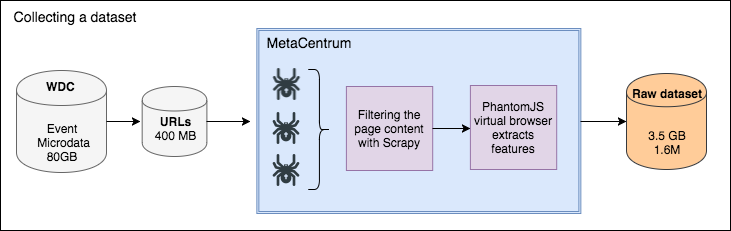
\includegraphics[width=1.0\textwidth]{dataset_collect}
\caption{The scheme of dataset collecting process}
\label{fig:collect}
\end{center}
\end{figure}
